
%(BEGIN_QUESTION)
% Copyright 2011, Tony R. Kuphaldt, released under the Creative Commons Attribution License (v 1.0)
% This means you may do almost anything with this work of mine, so long as you give me proper credit

Three level-sensing instruments measure the same liquid level at the bottom of this fractionation tower (LT-38a, LT-38b, and LT-38c), but their measurements do not agree.  An operator calls you to investigate, showing you on the control system display how LT-38a registers 46.2\%, LT-38b registers 45.9\%, and LT-38c registers 58.5\%: 

$$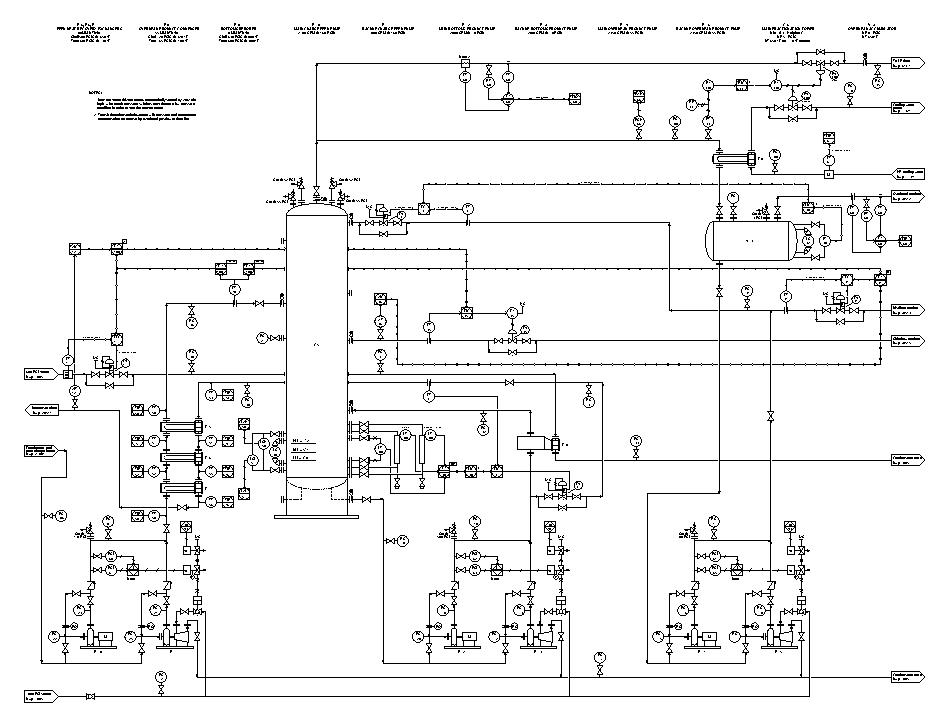
\includegraphics[width=15.5cm]{i0001rx02.eps}$$

Your first test is to have the operator take a sample of liquid from the bottom of the tower and analyze its density to see if it is within spec.  The operator does this, and it appears the density is exactly what it should be for normal tower operation.  First, explain why this was a useful test to do, and what you would have expected the density to test at (i.e. less than normal or greater than normal?) had this been the problem.

Next, identify a condition that could account for the discrepancy in these transmitter indications, and also determine what your diagnostic step would be after taking the density sample.

\vskip 20pt \vbox{\hrule \hbox{\strut \vrule{} {\bf Suggestions for Socratic discussion} \vrule} \hrule}

\begin{itemize}
\item{} Why do you suppose three different instruments are used to measure the same liquid level in this application?
\item{} Identify the function of LY-38.
\item{} If the tower bottoms product happened to be denser than it should be, what effect would this have on all three level transmitters' readings?
\item{} If the tower bottoms product temperature happens to increase dramatically, what effect will this have on all three level transmitters' readings?
\end{itemize}

\underbar{file i03427}
%(END_QUESTION)





%(BEGIN_ANSWER)

That first step was good because a wrong density could explain a false reading on both LT-38a and LT-38b.

%(END_ANSWER)





%(BEGIN_NOTES)

Since both LT-38a (hydrostatic) and LT-38b (displacer) are density-dependent instruments, the first test was good to see if an abnormal density could account for both these instruments reading differently than LT-38c (magnetostrictive float).  With LT-38a and LT-38b both reading less liquid level than LT-38c, a plausible cause would be a liquid density that is {\it lower} than normal (i.e. generates less hydrostatic pressure and less buoyant force than it should for a given height).

\vskip 10pt

A good next test would be to manually move the level up and down (controller in manual mode) to see if all three instruments respond.  This would test for the possibility of the float in LT-38c being stuck.  Alternatively, one could read the trend graph for all three instruments to compare how ``active'' LT-38c's trend was compared to the others.

\vskip 20pt \vbox{\hrule \hbox{\strut \vrule{} {\bf Virtual Troubleshooting} \vrule} \hrule}

This question is a good candidate for a ``Virtual Troubleshooting'' exercise.  Presenting the diagram to students, you first imagine in your own mind a particular fault in the system.  Then, you present one or more symptoms of that fault (something noticeable by an operator or other user of the system).  Students then propose various diagnostic tests to perform on this system to identify the nature and location of the fault, as though they were technicians trying to troubleshoot the problem.  Your job is to tell them what the result(s) would be for each of the proposed diagnostic tests, documenting those results where all the students can see.

During and after the exercise, it is good to ask students follow-up questions such as:

\begin{itemize}
\item{} What does the result of the last diagnostic test tell you about the fault?
\item{} Suppose the results of the last diagnostic test were different.  What then would that result tell you about the fault?
\item{} Is the last diagnostic test the best one we could do?
\item{} What would be the ideal order of tests, to diagnose the problem in as few steps as possible?
\end{itemize}

%INDEX% Measurement, level: troubleshooting
%INDEX% Process: distillation, generic (realistic P&ID shown)

%(END_NOTES)

